\subsection{Erstellung von Referenzpunkten für die KI}
Zunächst wird auf einen Mechanismus eingegangen, der die Referenzpunkte anhand des kompletten Spielfeldes ermittelt. Da dies jedoch ein sehr statischer Mechanismus ist, ist zusätzlich ein Algorithmus entwickelt worden, der die Referenzpunkte in einem angegebenen Radius berechnet. Dies dient der Motivation, dass sich ein menschlicher Spieler auch nur Teilausschnitte des Spielfelds betrachtet und sich der Algorithmus zur Berechnung der Referenzpunkte stärker einer KI ähneln soll. Dies wird im anschließenden Abschnitte ausführlich erläutert.\\
\subsubsection{Berechnung der Referenzpunkte anhand des kompletten Spielfeldes}
Damit ein Algorithmus bzw. eine KI ermitteln kann, ob sich das eigene Fahrzeug gerade auf einem richtigen Weg zum Ziel befindet, müssen folgende Punkte auf jeden Fall berücksichtigt werden:
\begin{enumerate}
\item \label{en-pkt1} Das Spielfeld muss von der Startposition aus einmal durchlaufen werden. Hierbei ist das Ziel, einen Ringschluss zum Start zu finden.
\item \label{en-pkt2} Bei Ecken ist es wichtig alle Richtungsmöglichkeiten zu prüfen.
\item \label{en-pkt3} Es ist zusätzlich ein Mechanismus, der auf Sackgassen reagiert, notwendig.
\item \label{en-pkt4} Nachdem das Spielfeld einmal durchlaufen ist, sollen die Referenzpunkte anhand der ermittelten Strecke gesetzt werden.
\end{enumerate}
Die Umsetzung dieser Punkte wird im Folgenden nacheinander erläutert. Dieser wesentliche Ablauf des Algorithmus ist in \autoref{fig:aktivity_refp} dargestellt.

\begin{figure}[h]
\centering
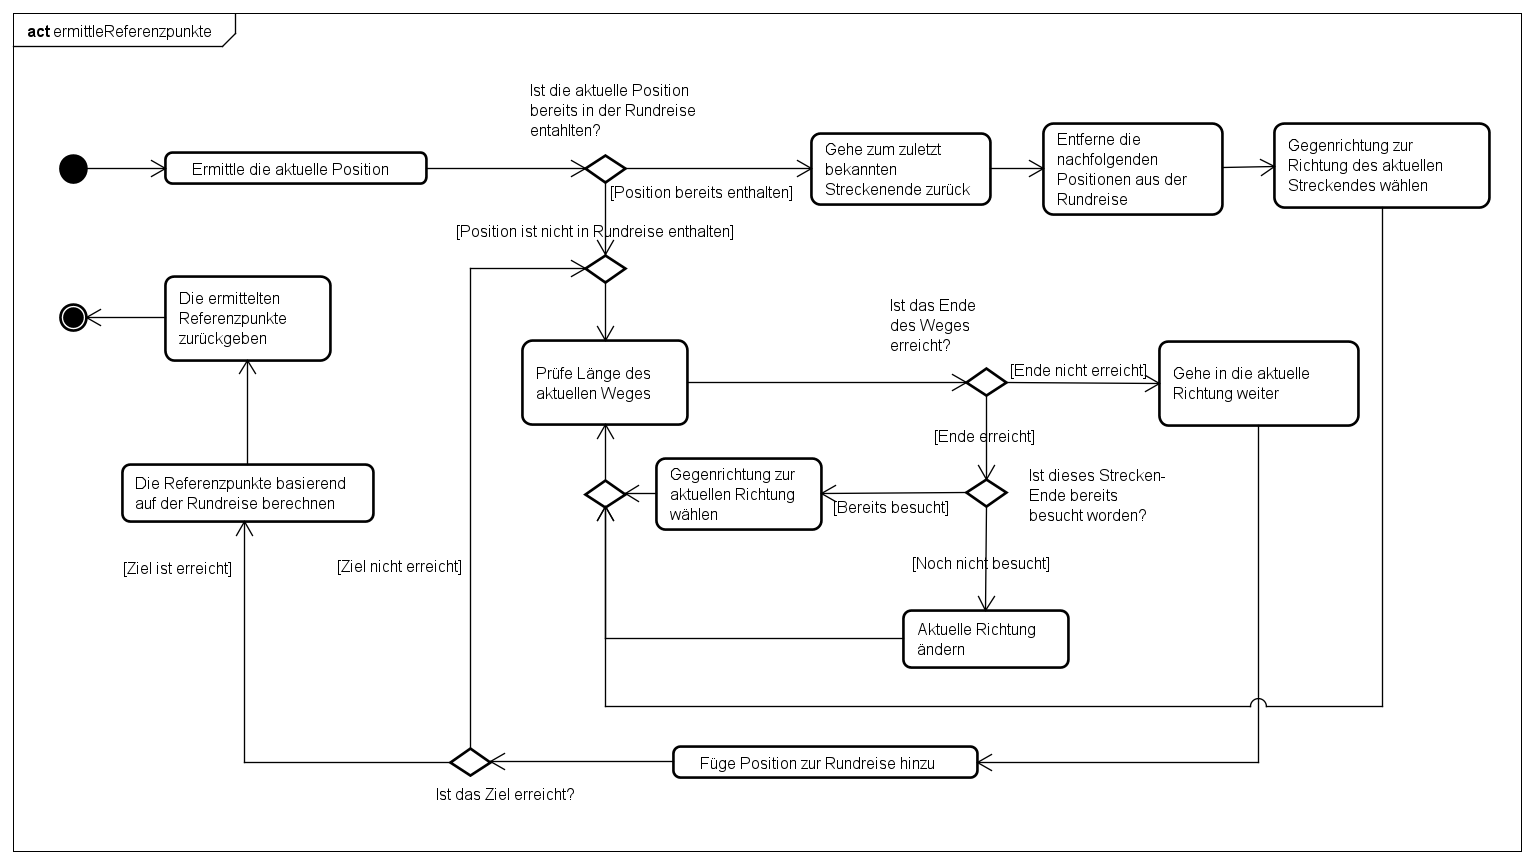
\includegraphics[scale=0.4]{pics/ermittleReferenzpunkte.png}
\caption{Ermittlung der Referenzpunkte}
\label{fig:aktivity_refp}
\end{figure}

\autoref{en-pkt1} prüft lediglich die Länge der aktuellen Fahrbahn bis zum Ende. Solange man sich auf einem akzeptierten Weg (z.B. Asphalt) befindet, wird in die aktuelle Richtung weitergegangen und diese Position wird zur Ergebnisstrecke, die den Weg von Ausgangsposition bis Ziel beschreibt, aufgenommen.\\
Ist das Streckenende erreicht, so wird mit \autoref{en-pkt2} die nächste Fahrtrichtung ermittelt. Da hier lediglich die Richtungen \glqq links\grqq{}, \glqq rechts\grqq{}, \glqq oben\grqq{} und \glqq unten\grqq{} berücksichtigt werden, ergeben sich folgende Fälle:
\begin{itemize}
\item Die ursprüngliche Richtung ist \glqq oben\grqq{} oder \glqq unten\grqq{}: Es kann lediglich nach \glqq links\grqq{} oder \glqq rechts\grqq{} weitergefahren werden, da der Algorithmus bereits aus der Gegenrichtung (z.B. ist bei \glqq oben\grqq{} die Gegenrichtung \glqq unten\grqq{}) gekommen ist.
\item Die ursprüngliche Richtung ist \glqq links\grqq{} oder \glqq rechts\grqq{}: Es kann lediglich nach \glqq oben\grqq{} oder \glqq unten\grqq{} weitergefahren werden.
\end{itemize}
Ist also der Algorithmus auf ein Straßenende gestoßen, so wird lediglich die Richtung gewechselt und \autoref{en-pkt1} wird fortgeführt.\\
Trifft der Algorithmus auf eine Ecke und entscheidet sich zuerst für die Richtung, in die nicht weitergegangen werden kann, so ist \autoref{en-pkt3} notwendig. Hierbei werden zusätzlich alle bereits erreichten Streckenenden gespeichert. Wird also ein Ende erreicht, das bereits besucht wurde, so wird in die Gegenrichtung zur aktuellen Richtung weitergefahren. Befindet sich also beispielsweise die aktuelle Position in einer Ecke, bei der man nach \glqq oben\grqq{} weiterfahren soll, der Algorithmus entscheidet sich jedoch zuerst nach \glqq unten\grqq{} weiterzufahren, so wird in diesem Fall, da die Ecke bereits einmal behandelt wurde, nach \glqq oben\grqq{} weitergefahren (nachdem zuvor die Strecke nach \glqq unten\grqq{} betrachtet wurde).\\
Als weiteren Mechanismus ist es notwendig auf bereits erreichte Positionen zu prüfen, da dies bedeuten würde, dass der Algorithmus einmal im Kreis gelaufen ist. In so einem Fall wird der aktuelle Weg solange zurückgelaufen, bis das zuletzt erreichte Straßenende erreicht wurde. Hierbei werden diese Positionen auch aus der Ergebnisstrecke entfernt. Ist das zuletzt bekannte Straßenende erreicht, so wird in die Gegenrichtung dieser Ecke weitergegangen. Mithilfe dieses Mechanismus wird der Kreis verlassen.\\
Ist das Zielfeld erreicht und somit ein Ringschluss gefunden worden, erfolgt \autoref{en-pkt4}. Hierbei gibt der Nutzer die Anzahl an zu verwendenden Referenzpunkten vor. Es wird die Ergebnisstrecke in diese Anzahl aufgeteilt und das jeweilige Sub-Streckenende wird als Referenzpunkt gewählt.\\
Somit ist der Algorithmus zur Berechnung der Referenzpunkte anhand des kompletten Spielfeldes ausführlich erläutert worden. Anschließend wird auf eine KI-ähnelnde Version desselben Algorithmus eingegangen.

\subsubsection{Berechnung der Referenzpunkte innerhalb eines vorgegebenen Radius}
Die Grundidee dieser Version ist ähnlich des zuvor erläuterten Algorithmus. Hier wird lediglich ein zusätzlicher Zähler eingesetzt, der auf den angegebenen Sicht-Radius überprüft. Dieser Zähler erhöht sich, wenn der Algorithmus eine Kachel in die aktuelle Richtung weitergeht. Befindet sich der Algorithmus auf dem Rückweg, da beispielsweise eine Sackgasse erreicht wurde, so werden diese Kacheln von dem Zähler abgezogen, da nun ein anderer Teil des Umfelds betrachtet wird. Ist das Maximum, also der angegebene Radius, erreicht, so wird die aktuelle Kachel automatisch als Referenzpunkt gewählt. Will der Anwender nun den nächsten Referenzpunkt, so wird an dem zuletzt ermittelten Referenzpunkt fortgesetzt und der Prozess wiederholt sich. Zusätzlich werden alle bereits ermittelten Referenzpunkte abgespeichert.\\
Erreicht nun der Algorithmus einmal das Ziel der Rennstrecke, so wird nicht mehr nach den nächsten Referenzpunkten simuliert, sondern die gespeicherten Referenzpunkte werden lediglich ausgegeben. Dies soll das Wissen der KI repräsentieren, dass der Algorithmus bei der Berechnung angesammelt hat.